\clearpage
\section{Arduino Quantum Receiver}

\begin{refsection}

\begin{tcolorbox}	
\begin{tabular}{p{2.75cm} p{0.2cm} p{10.5cm}} 	
\textbf{Student Name}  &:&  Andr\'e Mourato (2018/01/28 - 2018/02/27)\\
\textbf{}  & &  Daniel Pereira (2017/09/01 - 2017/11/16)\\
\textbf{Goal}          &:& Estimate the BER in a Binary Phase Shift Keying optical transmission system with additive white Gaussian noise. Comparison with theoretical results.\\
\textbf{Directory}              &:& sdf/arduino\_quantum\_rx
\end{tabular}
\end{tcolorbox}

Binary Phase Shift Keying (BPSK) is the simplest form of Phase Shift Keying (PSK), in which binary information is encoded into a two state constellation with the states being separated by a phase shift of $\pi$ (see Figure~\ref{fig:BPSKConst}).

\begin{figure}[h]
\centering
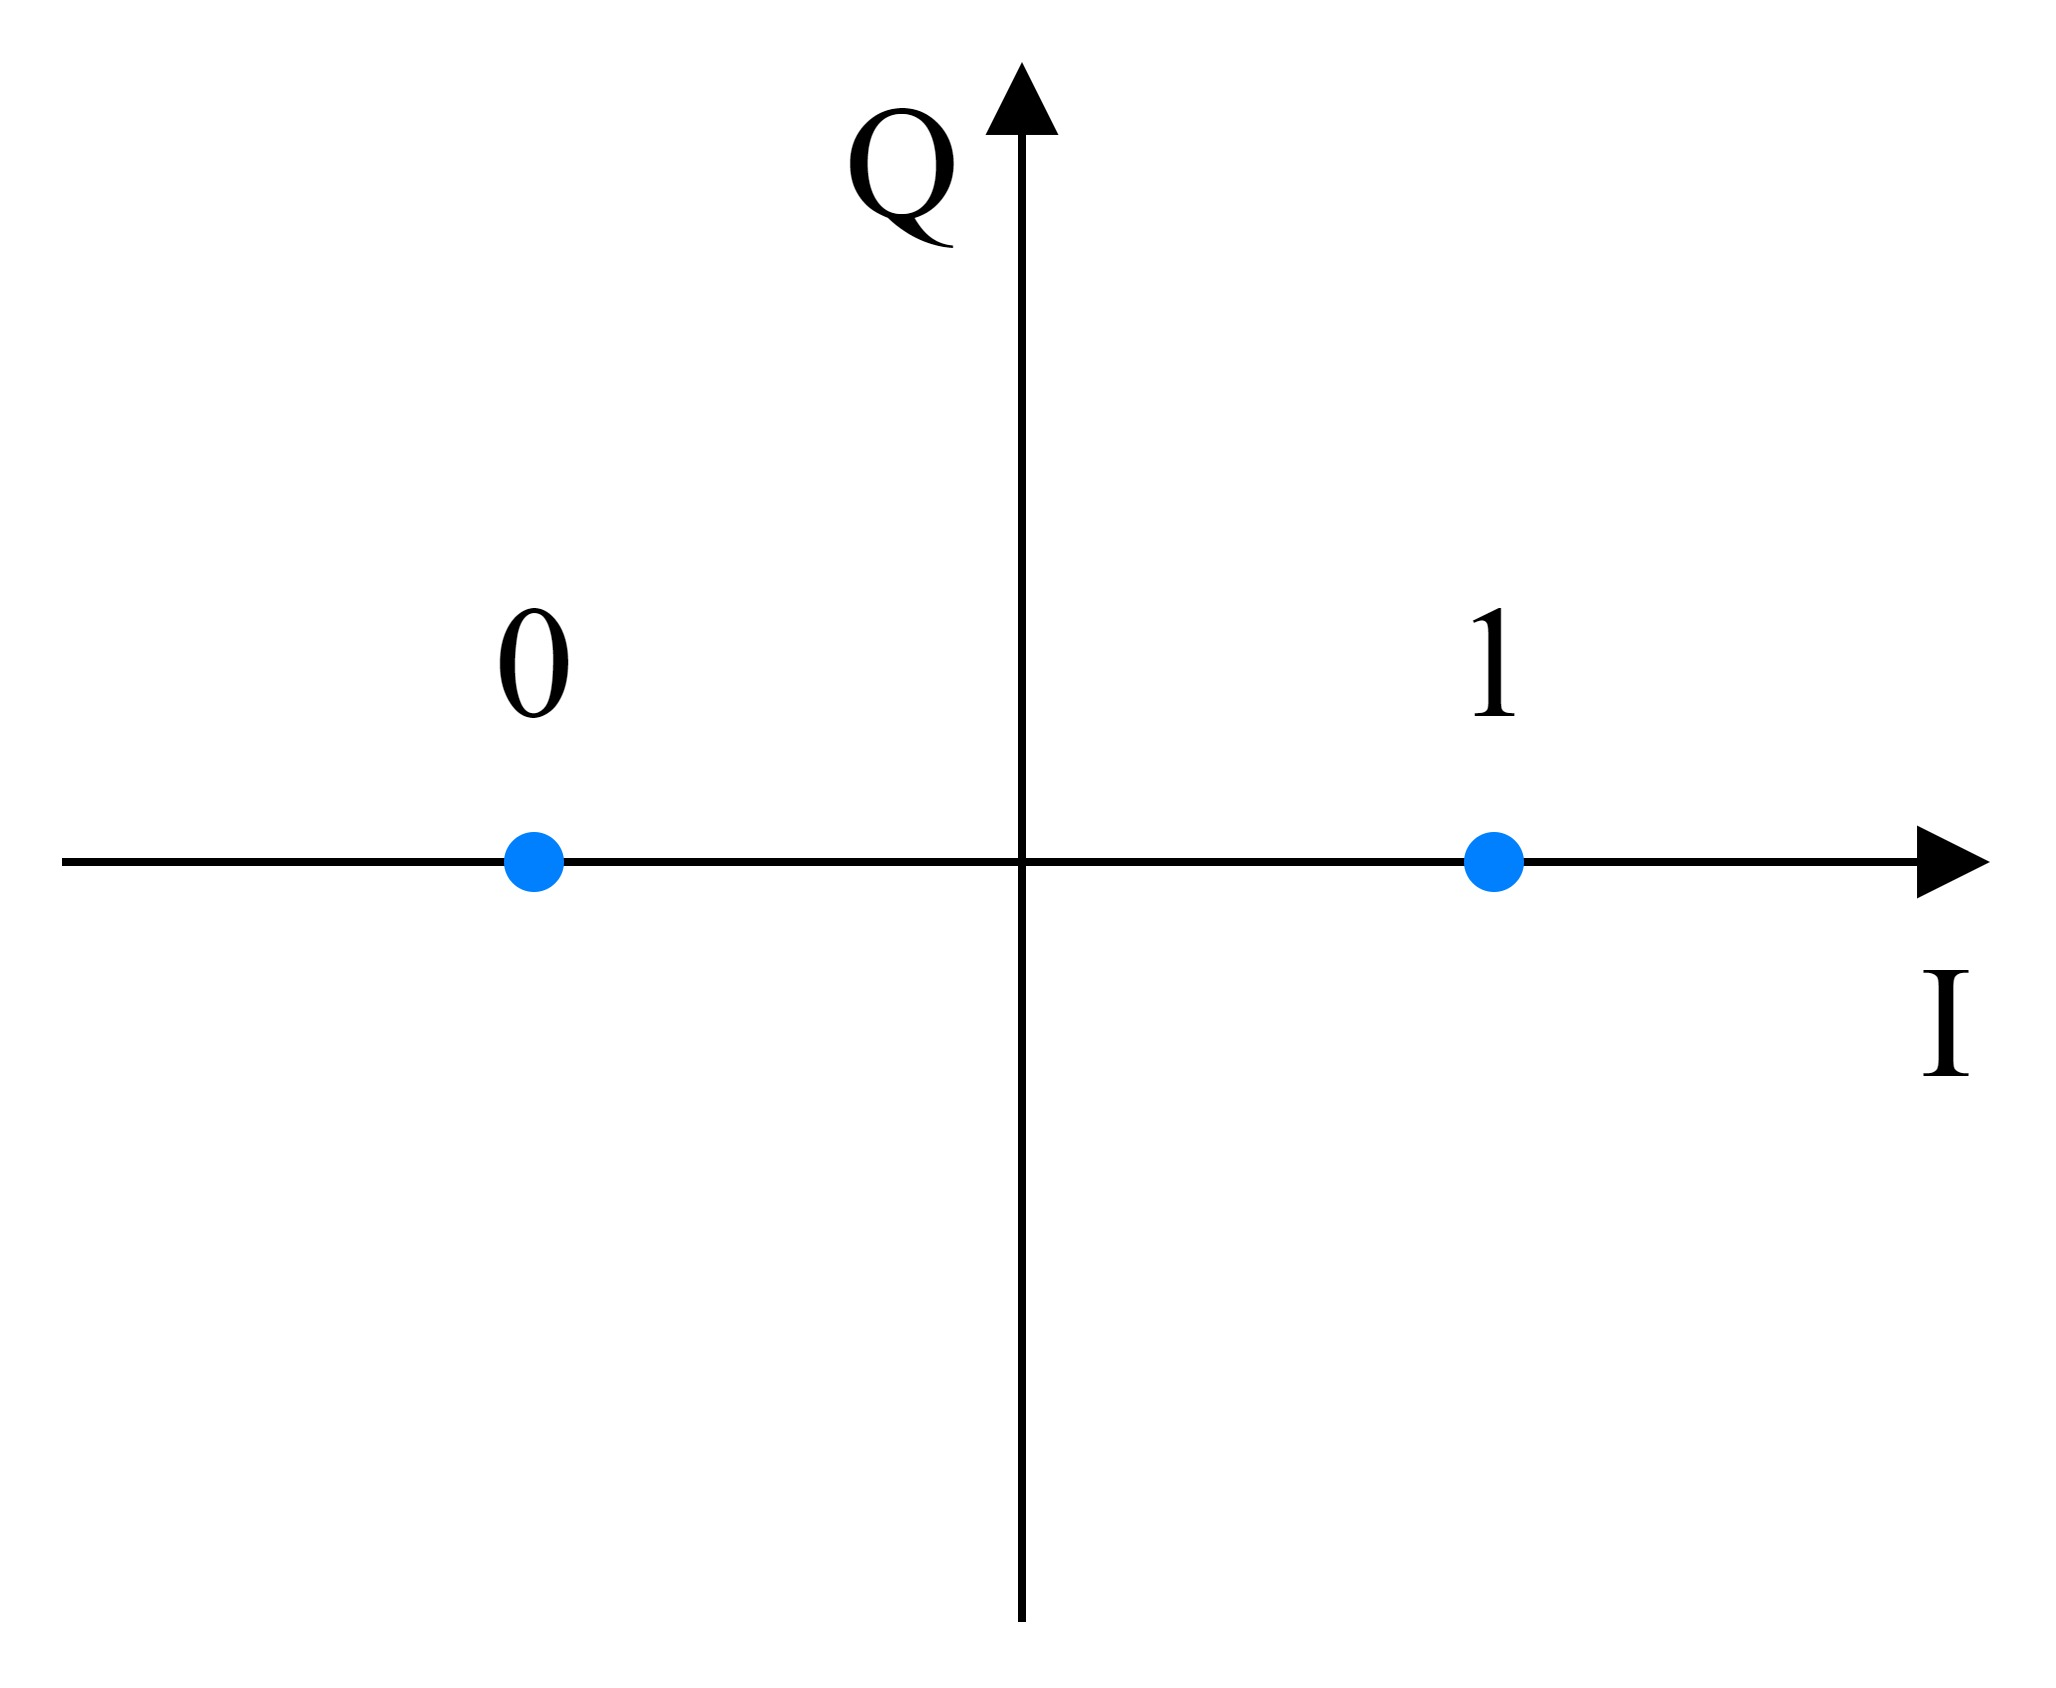
\includegraphics[width=.4\linewidth]{./sdf/arduino_quantum_rx/figures/bpskconstellation.jpg}
\caption{BPSK symbol constellation.}
\label{fig:BPSKConst}
\end{figure}

\par
White noise is a random signal with equal intensity at all frequencies, having a constant power spectral density. White noise is said to be Gaussian (WGN) if its samples follow a normal distribution with zero mean and a certain variance $\sigma^2$. For WGN its spectral density equals its variance. For the purpose of this work, additive WGN is used to model thermal noise at the receivers.
\par
The purpose of this system is to simulate BPSK transmission in back-to-back configuration with additive WGN at the receiver and to perform an accurate estimation of the BER and validate the estimation using theoretical values.

\subsection{Theoretical Analysis}

The output of the system with added gaussian noise follows a normal distribution, whose first probabilistic moment can be readily obtained by knowledge of the optical power of the received signal and local oscillator,
\begin{equation}\label{eq:mu1}
m_i=2\sqrt{P_LP_S}G_{ele}\cos(\Delta\theta_i),
\end{equation}
where $P_L$ and $P_S$ are the optical powers, in watts, of the local oscillator and signal, respectively, $G_{ele}$ is the gain of the trans-impedance amplifier in the coherent receiver and $\Delta\theta_i$ is the phase difference between the local oscillator and the signal, for BPSK this takes the values $\pi$ and 0, in which case~\eqref{eq:mu1} can be reduced to,
\begin{equation}
m_i=(-1)^{i+1}2\sqrt{P_LP_S}G_{ele},~i=0,~1.
\end{equation}
The second moment is directly chosen by inputting the spectral density of the noise $\sigma^2$, and thus is known \textit{a priori}.
\par
Both probabilist moments being known, the probability distribution of measurement results is given by a simple normal distribution,
\begin{equation}
f(x)=\frac{1}{\sqrt{2\pi}\sigma}e^{-\frac{(x-m_i)^2}{2\sigma^2}}.
\end{equation}
The BER is calculated in the following manner,
\begin{equation}
BER=\frac{1}{2}\int_0^{+\infty}f(x|\Delta\theta=\pi)\text{d}x+\frac{1}{2}\int^0_{-\infty}f(x|\Delta\theta=0)\text{d}x,
\end{equation}
given the symmetry of the system, this can be simplified to,
\begin{equation}\label{eq:BERtheoretical}
BER=\int_0^{+\infty}f(x|\Delta\theta=\pi)\text{d}x=\frac{1}{2}\text{erfc}\left(\frac{-m_0}{\sqrt{2}\sigma}\right)
\end{equation}




% bibliographic references for the section ----------------------------
\clearpage
\printbibliography[heading=subbibliography]
\end{refsection}
\addcontentsline{toc}{subsection}{Bibliography}
\cleardoublepage
% ---------------------------------------------------------------------
